\begin{problem}[1.2.11]
  Solve the equation $z^2 + z + 1 = 0$ for $z = (x, y)$ by writing
  \[%
    (x, y)(x, y) + (x, y) + (1, 0) = (0, 0)
  ,\]%
  and then solving a pair of simultaneous equations in $x$ and $y$.

  \textit{Suggestion:} Use the fact that no real number $x$ satisfies the given
  equation to show that $y \ne 0$.

  Ans. $\displaystyle z = \left(-\frac{1}{2}, \pm \frac{\sqrt{3}}{2}\right)$.
\end{problem}

\begin{proof}[Solution]
  Expanding the left-hand side and simplifying, we get
  \begin{alignat*}{3}
    z^2 + z + 1 = 0 &\implies (x^2 - y^2, 2xy) + (x, y) + (1, 0) &&= (0, 0) \\
                    &\implies (x^2 - y^2 + x + 1, 2xy + y) &&= (0, 0)
  .\end{alignat*}
  Therefore, we have the system of equations
  \begin{align*}
    x^2 - y^2 + x + 1 &= 0 \\
    2xy + y &= 0
  .\end{align*}
  From the second equation, we can factor out $y$ to get $y(2x + 1) = 0$. This
  gives us two cases to consider: either $y = 0$ or $2x + 1 = 0$.

  If $y = 0$, then substituting it back into the first equation gives us
  \[%
    x^2 + x + 1 = 0
  ,\]%
  which doesn't have any real solutions, as the discriminant is negative.
  Therefore, we must have $y \ne 0$.

  In the case where $2x + 1 = 0$, we can solve for $x$ to get $x =
  -\sfrac{1}{2}$. Substituting this value into the first equation gives us
  \begin{align*}
    0 &= \left(-\frac{1}{2}\right)^2 - y^2 - \frac{1}{2} + 1 \\
    0 &= \frac{1}{4} - y^2 - \frac{1}{2} + 1 \\
    0 &= -y^2 + \frac{3}{4} \\
    y^2 &= \frac{3}{4} \\
    y &= \pm\frac{\sqrt{3}}{2}
  .\end{align*}

  Thus, the solutions to the equation $z^2 + z + 1 = 0$ are
  \[%
    z = \left(-\frac{1}{2}, \pm \frac{\sqrt{3}}{2}\right) = -\frac{1}{2} \pm\frac{\sqrt{3}}{2}i
  .\qedhere\]%
\end{proof}

\begin{problem}[1.3.1]
  Reduce each of these quantities to a real number
  \[%
    \textrm{(i)}~\frac{1 + 2i}{3 - 4i} + \frac{2 - i}{5i}; \quad\quad \textrm{(ii)}~\frac{5i}{(1 - i)(2 - i)(3 - i)}; \quad\quad \textrm{(iii)}~(1 - i)^4
  .\]%
  Ans. (i) $-\sfrac{2}{5}$, (ii) $-\sfrac{1}{2}$, (iii) $-4$.
\end{problem}

\begin{proof}[Solution to (i)]
  Multiplying the numerator and denominator of the first term by the conjugate
  of the denominator, we have
  \[%
    \frac{1 + 2i}{3 - 4i} = \frac{(1 + 2i)(3 + 4i)}{(3 - 4i)(3 + 4i)} = \frac{3 + 4i + 6i - 8}{9 + 16} = \frac{-5 + 10i}{25} = -\frac{1}{5} + \frac{2}{5} i
  .\]%
  Now, we can simplify the second term
  \[%
    \frac{2 - i}{5i} = \frac{(2 - i)(-i)}{5i(-i)} = \frac{-2i - 1}{5} = -\frac{1}{5} - \frac{2}{5} i
  .\]%
  Adding these two results together, we have
  \[%
    \frac{1 + 2i}{3 - 4i} + \frac{2 - i}{5i} = \left(-\frac{1}{5} + \frac{2}{5} i\right) + \left(-\frac{1}{5} - \frac{2}{5} i\right) = -\frac{2}{5}
  .\qedhere\]%
\end{proof}

\begin{proof}[Solution to (ii)]
  Expanding the denominator, we have
  \[%
    \frac{5i}{(1 - i)(2 - i)(3 - i)} = \frac{5i}{(1 - 3i)(3 - i)} = -\frac{5i}{10i} = -\frac{1}{2}
  .\qedhere\]%
\end{proof}

\begin{proof}[Solution to (iii)]
  Expanding the polynomial $(1 - i)^2$, we have
  \[%
    (1 - i)^2 = (1 - i)(1 - i) = 1 - 2i + i^2 = 1 - 2i - 1 = -2i
  .\]%
  Now, we can expand $(1 - i)^4$ as follows
  \[%
    (1 - i)^4 = (1 - i)^2(1 - i)^2 = (-2i)(-2i) = 4i^2 = -4
  .\qedhere\]%
\end{proof}

\begin{problem}[1.4.1]
  Locate the numbers $z_1 + z_2$ and $z_1 - z_2$ vertically when
  \begin{alignat*}{6}
    &\textrm{(i)}~&&z_1 = 2i, \quad &&z_2 = \frac{2}{3} - i; \quad\quad&&\textrm{(ii)}~z_1 = (-\sqrt{3}, 1), \quad &&z_2 = (\sqrt{3}, 0); \\
    &\textrm{(iii)}~&&z_1 = (-3, 1), \quad &&z_2 = (1, 4); \quad\quad&&\textrm{(iv)}~z_1 = x_1 + y_1i, \quad &&z_2 = x_1 - y_1i
  .\end{alignat*}
\end{problem}

\begin{proof}[Solution to (i)]
  Graphing the complex numbers $z_1 = 2i$ and $z_2 = \frac{2}{3} - i$ on the
  complex plane, we have

  \begin{multicols}{2}
    \begin{center}
      \begin{tikzpicture}[scale=1.5]
        % Draw axes
        \draw[->, thick] (-1.5, 0) -- (2, 0) node[right] {$\Re(z)$};
        \draw[->, thick] (0, -1.5) -- (0, 3.5) node[above] {$\Im(z)$};

        % Dashed lines for visualization
        \draw[dashed,-] (2/3,-1) -- (2/3,1);
        \draw[dashed,-] (0,2) -- (2/3,1);
        \draw[dashed,-] (-2/3,3) -- (0,2);
        \draw[dashed,-] (-2/3,3) -- (-2/3,1);

        % Plot z1 = 2i
        \draw[red,->,thick] (0,0) -- (0,2) node[midway,right] {$z_1$};

        % Plot z2 = 2/3 - i
        \draw[blue,->,thick] (0,0) -- (2/3,-1) node[midway,below left] {$z_2$};

        % Plot -z2 = -2/3 + i
        \draw[blue,->,thick] (0,0) -- (-2/3,1) node[midway,left] {$-z_2$};

        % Plot z1 + z2 = 2/3 + i
        \draw[green,->,thick] (0,0) -- (2/3,1) node[midway,below,sloped] {$z_1 + z_2$};

        % Plot z1 - z2 = -2/3 + 3i
        \draw[orange,->,thick] (0,0) -- (-2/3,3) node[midway,below,sloped] {$z_1 - z_2$};
      \end{tikzpicture}
    \end{center}
    \columnbreak
    \noindent In this case, we can compute
    \[%
      z_1 + z_2 = \left(0 + 2i\right) + \left(\frac{2}{3} - i\right) = \frac{2}{3} + i
    .\]%
    This gives us the point $(\sfrac{2}{3}, 1)$. Similarly, we can compute
    \[%
      z_1 - z_2 = z_1 + (-z_2) = \left(0 + 2i\right) + \left(-\frac{2}{3} + i\right) = -\frac{2}{3} + 3i
    .\]%
    This gives us the point $(-\sfrac{2}{3}, 3)$. \qedhere
  \end{multicols}
\end{proof}

\begin{proof}[Solution to (ii)]
  Graphing the complex numbers $z_1 = (-\sqrt{3}, 1)$ and $z_2 = (\sqrt{3}, 0)$
  on the complex plane, we have
  \begin{center}
    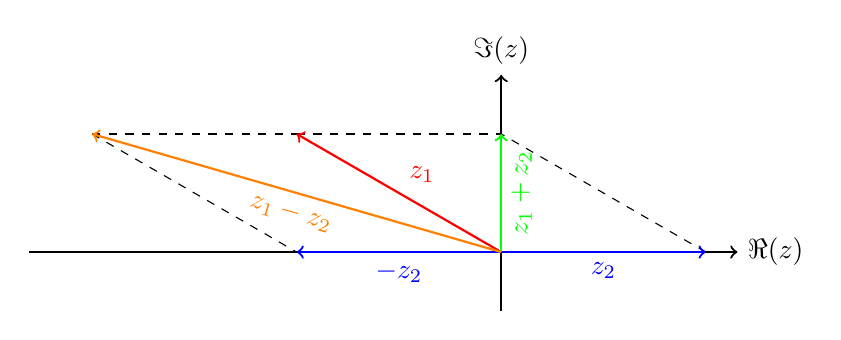
\begin{tikzpicture}[scale=1.5]
      % Draw axes
      \draw[->, thick] (-4, 0) -- (2, 0) node[right] {$\Re(z)$};
      \draw[->, thick] (0, -0.5) -- (0, 1.5) node[above] {$\Im(z)$};

      % Dashed lines for visualization
      \draw[dashed,-] (-1.732,1) -- (0,1);
      \draw[dashed,-] (1.732,0) -- (0,1);
      \draw[dashed,-] (-2*1.732,1) -- (-1.732,1);
      \draw[dashed,-] (-2*1.732,1) -- (-1.732,0);

      % Plot z1 = (-sqrt(3),1)
      \draw[red,->,thick] (0,0) -- (-1.732,1) node[midway,above right] {$z_1$};

      % Plot z2 = (sqrt(3),0)
      \draw[blue,->,thick] (0,0) -- (1.732,0) node[midway,below] {$z_2$};

      % Plot -z2 = (-sqrt(3),0)
      \draw[blue,->,thick] (0,0) -- (-1.732,0) node[midway,below] {$-z_2$};

      % Plot z1 + z2 = (0,1)
      \draw[green,->,thick] (0,0) -- (0,1) node[midway,below,sloped] {$z_1 + z_2$};

      % Plot z1 - z2 = (-2sqrt(3),1)
      \draw[orange,->,thick] (0,0) -- (-2*1.732,1) node[midway,below,sloped] {$z_1 - z_2$};
    \end{tikzpicture}
  \end{center}
  In this case, we can compute
  \[%
    z_1 + z_2 = \left(-\sqrt{3}, 1\right) + \left(\sqrt{3}, 0\right) = (0, 1)
  .\]%
  This gives us the point $(0, 1)$. Similarly, we can compute
  \[%
    z_1 - z_2 = z_1 + (-z_2) = \left(-\sqrt{3}, 1\right) + \left(-\sqrt{3}, 0\right) = (-2\sqrt{3}, 1)
  .\]%
  This gives us the point $(-2\sqrt{3}, 1)$. \qedhere
\end{proof}

\begin{proof}[Solution to (iii)]
  Graphing the complex numbers $z_1 = (-3, 1)$ and $z_2 = (1, 4)$ on the complex
  plane, we have

  \begin{multicols}{2}
    \begin{center}
      \begin{tikzpicture}[scale=1.5]
        % Draw axes
        \draw[->, thick] (-3, 0) -- (1.5, 0) node[right] {$\Re(z)$};
        \draw[->, thick] (0, -2.5) -- (0, 3.5) node[above] {$\Im(z)$};

        % Dashed lines for visualization
        \draw[dashed,-] (-3/2,1/2) -- (-3/2+1,1/2+2);
        \draw[dashed,-] (1,2) -- (-3/2+1,1/2+2);
        \draw[dashed,-] (-3/2,1/2) -- (-3/2-1,1/2-2);
        \draw[dashed,-] (-1,-2) -- (-3/2-1,1/2-2);

        % Plot z1 = (-3,1)
        \draw[red,->,thick] (0,0) -- (-3/2,1/2) node[midway,above right] {$z_1$};

        % Plot z2 = (1,4)
        \draw[blue,->,thick] (0,0) -- (1,2) node[midway,right] {$z_2$};

        % Plot -z2 = (-1,4)
        \draw[blue,->,thick] (0,0) -- (-1,-2) node[midway,right] {$-z_2$};

        % Plot z1 + z2 = (0,1)
        \draw[green,->,thick] (0,0) -- (-3/2+1,1/2+2) node[midway,below,sloped] {$z_1 + z_2$};

        % Plot z1 - z2 = (-2sqrt(3),1)
        \draw[orange,->,thick] (0,0) -- (-3/2-1,1/2-2) node[midway,below,sloped] {$z_1 - z_2$};
      \end{tikzpicture}
    \end{center}
    \columnbreak
    \noindent In this case, we can compute
    \[%
      z_1 + z_2 = \left(-3, 1\right) + \left(1, 4\right) = (-2, 5)
    .\]%
    This gives us the point $(-2, 5)$. Similarly, we can compute
    \[%
      z_1 - z_2 = z_1 + (-z_2) = \left(-3, 1\right) + \left(-1, -4\right) = (-4, -3)
    .\]%
    This gives us the point $(-4, -3)$. \qedhere
  \end{multicols}
\end{proof}

\begin{proof}[Solution to (iv)]
  Graphing the complex numbers $z_1 = x_1 + y_1i$ and $z_2 = x_1 - y_1i$ on the
  complex plane, we have

  \newpage

  \begin{multicols}{2}
    \begin{center}
      \begin{tikzpicture}[scale=1.5]
        % Draw axes
        \draw[->, thick] (-1.5, 0) -- (2.5, 0) node[right] {$\Re(z)$};
        \draw[->, thick] (0, -2.5) -- (0, 4.5) node[above] {$\Im(z)$};

        % let x1 = 1 for instance
        % let y1 = 2 for instance

        % Dashed lines for visualization
        \draw[dashed,-] (1,2) -- (2,0);
        \draw[dashed,-] (1,-2) -- (2,0);
        \draw[dashed,-] (1,2) -- (0,4);
        \draw[dashed,-] (-1,2) -- (0,4);

        % Plot z1 = (1, 2)
        \draw[red,->,thick] (0,0) -- (1,2) node[midway,above right] {$z_1$};

        % Plot z2 = (1, -2)
        \draw[blue,->,thick] (0,0) -- (1,-2) node[midway,right] {$z_2$};

        % Plot -z2 = (-1,2)
        \draw[blue,->,thick] (0,0) -- (-1,2) node[midway,right] {$-z_2$};

        % Plot z1 + z2 = (2,0)
        \draw[green,->,thick] (0,0) -- (2,0) node[midway,below,sloped] {$z_1 + z_2$};

        % Plot z1 - z2 = (0,4)
        \draw[orange,->,thick] (0,0) -- (0,4) node[midway,below,sloped] {$z_1 - z_2$};
      \end{tikzpicture}
    \end{center}
    \columnbreak
    In this case, we can compute
    \[%
      z_1 + z_2 = \left(x_1 + y_1i\right) + \left(x_1 - y_1i\right) = (2x_1 + 0i)
    .\]%
    This gives us the point $(2x_1, 0)$. Similarly, we can compute
    \[%
      z_1 - z_2 = z_1 + (-z_2) = \left(x_1 + y_1i\right) + \left(x_1 - y_1i\right) = (0, 2y_1)
    .\]%
    This gives us the point $(0, 2y_1)$. \qedhere
  \end{multicols}
\end{proof}

\begin{problem}[1.4.4]
  Verify that $\sqrt{2}\lvert z \rvert \ge \lvert \Re(z) \rvert + \lvert \Im(z)
  \rvert$.

  \textit{Suggestion:} Reduce this inequality to $(\lvert x \rvert - \lvert y
  \rvert)^2 \ge 0$.
\end{problem}

\begin{proof}[Solution]
  We know that $\Re(z) = \lvert x \rvert$ and $\Im(z) = \lvert y \rvert$. We
  also know that $\lvert z \rvert = \sqrt{x^2 + y^2}$. Therefore, we can rewrite
  the inequality as
  \begin{align*}
    \phantom{\implies}\quad&2\lvert z \rvert \ge \lvert \Re(z) \rvert + \lvert \Im(z) \rvert \\
    \implies\quad&2\sqrt{x^2 + y^2} \ge \lvert x \rvert + \lvert y \rvert \\
    \implies\quad&2(x^2 + y^2) \ge (\lvert x \rvert + \lvert y \rvert)^2 \\
    \implies\quad&2(x^2 + y^2) \ge x^2 + 2\lvert x \rvert \lvert y \rvert + y^2 \\
    \implies\quad&2x^2 + 2y^2 - x^2 - 2\lvert x \rvert \lvert y \rvert - y^2 \ge 0 \\
    \implies\quad&(x^2 + y^2) - 2\lvert x \rvert \lvert y \rvert \ge 0 \\
    \implies\quad&(x - \lvert y \rvert)(x + \lvert y \rvert) \ge 0
  .\end{align*}
  Since $x^2 + y^2 = \lvert x \rvert^2 + \lvert y \rvert^2$, we can re-write the
  inequality as
  \begin{align*}
    \phantom{\implies}\quad&(x - \lvert y \rvert)(x + \lvert y \rvert) \ge 0 \\
    \implies\quad&(\lvert x \rvert - \lvert y \rvert)^2 \ge 0
  .\end{align*}
  Therefore, we have $(\lvert x \rvert - \lvert y \rvert)^2 \ge 0$, which is
  always true. This means that $\sqrt{2}\lvert z \rvert \ge \lvert \Re(z) \rvert
  + \lvert \Im(z) \rvert$ is true for all complex numbers $z$.
\end{proof}

\begin{problem}[1.4.6]
  Using the fact that $\lvert z_1 - z_2 \rvert$ is the distance between two
  points $z_1$ and $z_2$, give a geometric argument that
  \begin{enumerate}
    \item $\lvert z - 4i \rvert + \lvert z + 4i \rvert = 10$ represents an
      ellipse whose foci are $(0, \pm 4)$.

    \item $\lvert z - 1 \rvert = \lvert z + i \rvert$ represents the line
      through the origin whose slope is $-1$.
  \end{enumerate}
\end{problem}

\begin{proof}[Solution to (i)]
  The modulus $\lvert z - 4i \rvert$ represents the Euclidean distance between
  the complex number $z$ and the point $4i$. Similarly, $\lvert z + 4i \rvert$
  represents the distance from $z$ to $-4i$.

  Since the sum of the distances from any point $z$ on the curve to the fixed
  points $(0, 4)$ and $(0, -4)$ is a constant, this satisfies the definition of
  an ellipse, where the sum of distances to the foci is constant.

  The foci are at $(0, \pm 4)$. The given sum of distances is $10$, which
  corresponds to $2a$ in the standard form of an ellipse equation. The foci are
  at a distance $c = 4$ from the center $(0, 0)$, and using the standard ellipse
  relation $a^2 = b^2 + c^2$, we get $a = 5$, $b = 3$, and $c = 4$. Thus, the
  ellipse has semi-major axis $a = 5$ and semi-minor axis $b = 3$.
\end{proof}

\begin{proof}[Solution to (ii)]
  The expression $\lvert z - 1 \rvert$ represents the distance from $z$ to $1$.
  The expression $\lvert z + i \rvert$ represents the distance from $z$ to $-i$.

  The equation states that any point $z = x + yi$ is equidistant from these two
  fixed points. The midpoint of $(1, 0)$ and $(0, -1)$ is
  \[%
    \left(\frac{1 + 0}{2}, \frac{0 + (-1)}{2}\right) = \left(\frac{1}{2}, -\frac{1}{2}\right)
  .\]%
  The slope of the segment joining $(1,0)$ and $(0,-1)$ is $m = 1$. The
  perpendicular bisector has a slope of $-1$, so its equation is
  \[%
    y + \frac{1}{2} = -1(x - \frac{1}{2}) \implies y = -x + 1
  .\]%
  Thus, the given equation represents the line through the origin with slope
  $-1$.
\end{proof}

\begin{problem}[1.5.1(iv)]
  Use properties of conjugates and moduli established in Sec. $5$ to show that
  \begin{enumerate}
    \item[(iv)] $\lvert (2\zb + 5)(\sqrt{2} - i) \rvert = \sqrt{3} \lvert 2z + 5
      \rvert$.
  \end{enumerate}
\end{problem}

\begin{proof}[Solution to (iv)]
  Expanding the left-hand side, we have
  \[%
    \lvert (2\zb + 5)(\sqrt{2} - i) \rvert = \lvert 2\zb + 5 \rvert \cdot \lvert \sqrt{2} - i \rvert
  .\]%
  Taking the norm of the complex number $\sqrt{2} - i$, we have
  \[%
    \lvert \sqrt{2} - i \rvert = \sqrt{(\sqrt{2})^2 + (-i)^2} = \sqrt{2 + 1} = \sqrt{3}
  .\]%
  Therefore, we have
  \[%
    \lvert (2\zb + 5)(\sqrt{2} - i) \rvert = \sqrt{3} \cdot \lvert 2\zb + 5 \rvert
  .\]%
  Since $\lvert z \rvert = \lvert \zb \rvert$, we can replace $\lvert 2\zb + 5
  \rvert$ with $\lvert 2z + 5 \rvert$ to get
  \[%
    \lvert (2\zb + 5)(\sqrt{2} - i) \rvert = \sqrt{3} \lvert 2z + 5 \rvert
  .\qedhere\]%
\end{proof}

\begin{problem}[1.5.10]
  Prove that
  \begin{enumerate}
    \item $z$ is real if and only if $\zb = z$.

    \item $z$ is either real or pure imaginary if and only if $\zb^2 = z^2$.
  \end{enumerate}
\end{problem}

\begin{proof}[Solution to (i)]
  Assume $z$ is real. This means that $z = x + 0i$ for some real number $x$. The
  complex conjugate of $z$ is $\zb = x - 0i = x$. Therefore, we have $\zb = z$.

  Conversely, assume $\zb = z$. This means that $z = x + yi$ and $\zb = x - yi$.
  By assumption, we have $\zb = z$ giving us $x + yi = x - yi$. This implies
  that $yi = -yi$, giving us $y = -y$. This only holds true if $y = 0$.
  Therefore, we have $z = x + 0i$ for some real number $x$. This means that $z$
  is real.

  Thus, $z$ is real if and only if $\zb = z$.
\end{proof}

\begin{proof}[Solution to (ii)]
  Assume $z$ is either real or pure imaginary. This gives us two cases, when $z$
  is real, $z = x + 0i$ for some real number $x$, and when $z$ is pure
  imaginary, $z = 0 + yi$ for some real number $y$. Notice that the first case
  is already proven in part (i), i.e., $z = \zb$, giving us $z^2 = \zb^2$. In
  the second case, we have $z = 0 + yi$ and $\zb = 0 - yi = -yi$. Therefore, we
  have $\zb^2 = (-yi)^2 = -y^2$. On the other hand, $z^2 = (0 + yi)^2 = -y^2$.
  Therefore, we have $\zb^2 = z^2$.

  Assume $\zb^2 = z^2$. Let $z = x + yi$ and $\zb = x - yi$. By assumption, we
  have
  \[%
    z^2 = \zb^2 \implies (x + yi)^2 = (x - yi)^2 \implies x^2 - y^2 + 2xyi = x^2 - y^2 - 2xyi
  .\]%
  Comparing the real parts, we have $x^2 - y^2 = x^2 - y^2$, which is always
  true. Comparing the imaginary parts, we have $2xy = -2xy$. This implies that
  $4xy = 0$. This means that either $x = 0$ or $y = 0$. If $x = 0$, then $z$ is
  pure imaginary. If $y = 0$, then $z$ is real. Therefore, $z$ is either real or
  pure imaginary.

  Thus, $z$ is either real or pure imaginary if and only if $\zb^2 = z^2$.
\end{proof}

\begin{problem}[1.5.14]
  Using expressions ($6$), Sec. $5$, for $\Re(z)$ and $\Im(z)$, show that the
  hyperbola $x^2 - y^2 = 1$ can be written as
  \[%
    z^2 + \zb^2 = 2
  .\]%
\end{problem}

\begin{proof}[Solution]
  Substituting $\Re(z)$ and $\Im(z)$ for $x$ and $y$ into the equation for the
  hyperbola, we have
  \[%
    x^2 - y^2 = 1 \implies \Re(z)^2 - \Im(z)^2 = 1 \implies \left(\frac{z + \zb}{2}\right)^2 - \left(\frac{z - \zb}{2i}\right)^2 = 1
  .\]%
  Expanding the left-hand side, we have
  \[%
    \left(\frac{z + \zb}{2}\right)^2 - \left(\frac{z - \zb}{2i}\right)^2 = \frac{(z + \zb)^2}{4} - \frac{(z - \zb)^2}{-4} = \frac{(z + \zb)^2 + (z - \zb)^2}{4}
  .\]%
  Therefore, we have $(z + \zb)^2 + (z - \zb)^2 = 4$. Expanding the squares, we
  have
  \begin{alignat*}{3}
    \phantom{\implies}&\quad z^2 + 2z\zb + \zb^2 + z^2 -2z\zb + \zb^2 &&= 4 \\
    \implies&\quad 2z^2 + 2\zb^2 &&= 4 \\
    \implies&\quad z^2 + \zb^2 &&= 2
  .\tag*{\qedhere}\end{alignat*}
\end{proof}

\begin{problem}[(Extra)]
  Given $a + bi$, $a$, $b$ are real numbers, find $c$ and $d$ such that $(c +
  di)^2 = a + bi$.
\end{problem}

\begin{proof}[Solution]
  Expanding the left-hand side, we have $(c + di)^2 = c^2 - d^2 + 2cdi$.
  Equating the real and imaginary parts, we get the following system of
  equations
  \begin{align*}
    c^2 - d^2 &= a \\
    2cd &= b
  .\end{align*}
  From the second equation, we can express $d$ in terms of $c$ and $b$ as
  follows
  \[%
    d = \frac{b}{2c}
  .\]%
  Plugging this expression for $d$ into the first equation, we have
  \begin{alignat*}{3}
    \phantom{\implies}\quad&c^2 - \left(\frac{b}{2c}\right)^2 &&= a \\
    \implies\quad&c^2 - \frac{b^2}{4c^2} &&= a \\
    \implies\quad&4c^4 - b^2 &&= 4ac^2 \\
    \implies\quad&4c^4 - 4ac^2 - b^2 &&= 0 \\
    \implies\quad&c^4 - ac^2 - \frac{b^2}{4} &&= 0
  .\end{alignat*}
\end{proof}
